\section{Qu'est-ce qu'un labyrinthe ?}
\subsection{Définition d'un labyrinthe}
Un labyrinthe est une structure complexe de passages reliés entre-eux. L’objectif du solveur est de passer d'un point de départ à un point d'arrivée, c'est-à-dire trouver le passage reliant ces deux points. Le labyrinthe est une énigme qui teste l'intelligence, la réflexion, et la rapidité d'exécutions du solveur. D'un point de vu mathématique, les labyrinthes peuvent êtres représentés comme étant des surfaces connexes. 


\subsection{Histoire et application}
Le mot labyrinthe trouve son origine dans la  mythologie grecque, c'était une structure constitué de galeries, construite par Dédale afin d'y enfermer le Minotaure.
Le divertissement et l'entraînement cérébral peuvent être considérés comme les principaux objectifs d'application d'un labyrinthe.
En ce qui concerne le domaine scientifique, les labyrinthes peuvent être vu comme des supports pour effectuer des démonstrations robotiques. Le concept de labyrinthe a permis la naissance de concours robotiques comme les compétitions Micromouses ou l'objectif est de résoudre une énigme (un labyrinthe) en ayant recours à différents algorithmes d'intelligence artificielle.
\section{Classification d'un labyrinthe} 
\label{sec:ProblematiqueConstructionLabyrinthe}
\paragraph{}
Les labyrinthes (et les algorithmes responsables de leur génération) peuvent être organisés selon trois critères de  classifications différents. Ces critères sont : la dimension, la topologie, et la tessellation. Un labyrinthe peut prendre un objet d'un de ses classes dans n'importe quelle combinaison.

\subsection{Dimension d'un labyrinthe}
La dimension d'un labyrinthe corresponds à l'espace dimensionnel couvert par le labyrinthe. Les labyrinthes peuvent êtres de dimensionnalité 2, 3 ou tout autre dimension supérieure.

\begin{figure*}[htp] 
    \centering
    \subfloat[Labyrinthe en 2 dimensions.]{%
        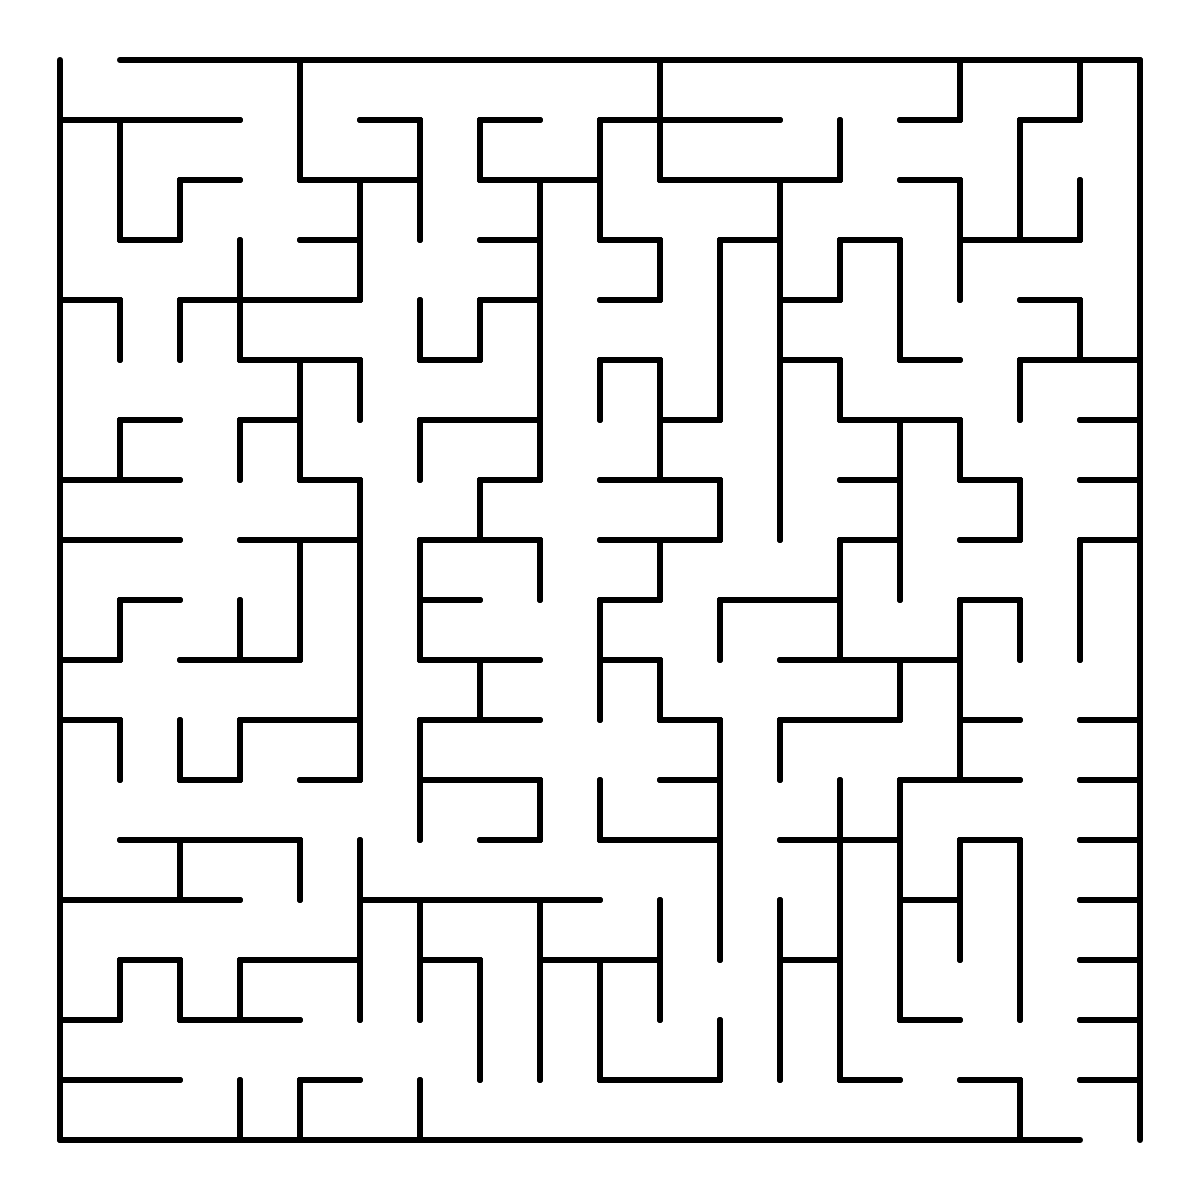
\includegraphics[width=0.35\textwidth]{report/pics/2D_maze.png}%
        \label{fig:a}%
        }%
    \hfill%
    \subfloat[Labyrinthe en 3 dimensions.]{%
        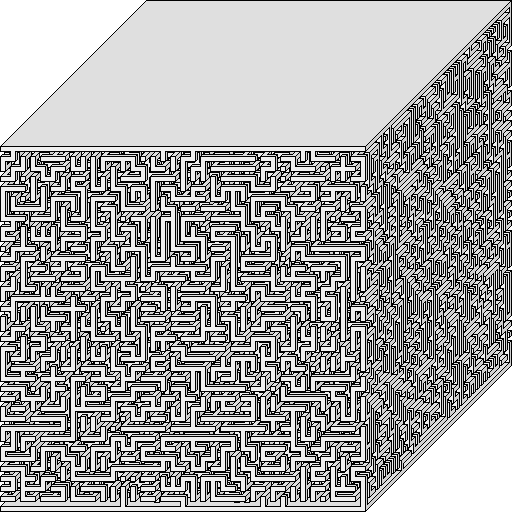
\includegraphics[width=0.35\textwidth]{pics/3D_maze.png}%
        \label{fig:b}%
        }%
    \caption{Exemple d'un labyrinthe 2D et d'un labyrinthe 3D}
\end{figure*}


\subsection{Tessellation d'un labyrinthe}
La classe de tessellation est la géométrie des cellules individuelles qui composent le labyrinthe. Il existe de nombreux types de tessellation, on citera notamment :
\begin{itemize}
\item\textbf{ Tesellation orthogonale :} Il s'agit d'une grille rectangulaire standard où les cellules ont des passages qui se coupent à angle droit formant des cellules sous forme de carrés.

\item\textbf{Tesellation delta :} Un labyrinthe à tessellation delta est un composé de triangles imbriqués, où chaque cellule peut avoir jusqu'à trois passages connectés.

\item\textbf{Tesellation theta :} Un labyrinthe à tessellation theta est composé de cercles concentriques. Les cellules ont généralement quatre connexions de passage possibles, mais peuvent en avoir plus en raison du plus grand nombre de cellules dans les anneaux externes.
\end{itemize}

\begin{figure*}[htp] 
    \centering
    \subfloat[Labyrinthe orthogonal.]{%
        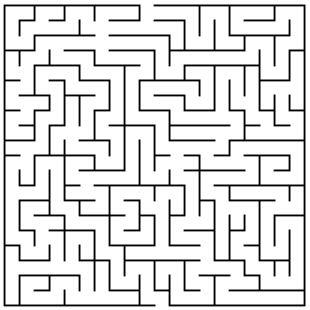
\includegraphics[width=0.27\textwidth]{report/pics/orthogonal_maze.png}%
        \label{fig:a}%
        }%
    \hfill%
    \subfloat[Labyrinthe delta.]{%
        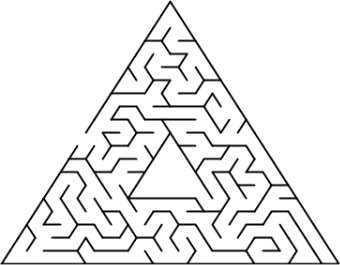
\includegraphics[width=0.3\textwidth]{report/pics/delta_maze.png}%
        \label{fig:b}%
        }%
        \hfill%
    \subfloat[Labyrinthe theta.]{%
        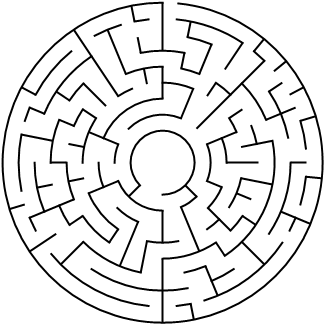
\includegraphics[width=0.3\textwidth]{report/pics/theta_maze.png}%
        \label{fig:c}%
        }%
    \caption{Exemple de labyrinthes avec différentes classes de tessellation.}
\end{figure*}


\subsection{Topologie d'un labyrinthe}
D’un point de vu mathématique, un labyrinthe est définie comme étant une surface connexe pouvant avoir deux types de topologies : topologie simple et topologie comportant des anneaux. Cette différence dans le type de topologie conduit à une distinction des labyrinthes en deux catégories : Les labyrinthes parfaits et les labyrinthes imparfaits.

\subsubsection{Labyrinthe parfait}
Afin qu'un labyrinthe soit labélisé comme étant parfait, ce dernier doit remplir deux conditions :
\begin{itemize}
\item Ne contient pas de cycles.
\item Il existe un unique chemin entre la cellule de départ et la cellule d’arrivée du labyrinthe.
\end{itemize}
Plus généralement, quelque soit deux cellules sélectionnées dans notre labyrinthe, le chemin entre ces deux cellules doit être unique.

\subsubsection{Labyrinthe imparfait}
Un labyrinthe qui ne remplit pas les conditions pour être labélisé comme parfait est dit imparfait. Les labyrinthes imparfaits peuvent donc contenir des boucles, des îlots ou des cellules inaccessibles.


\begin{figure*}[htp] 
    \centering
    \subfloat[Labyrinthe parfait.]{%
        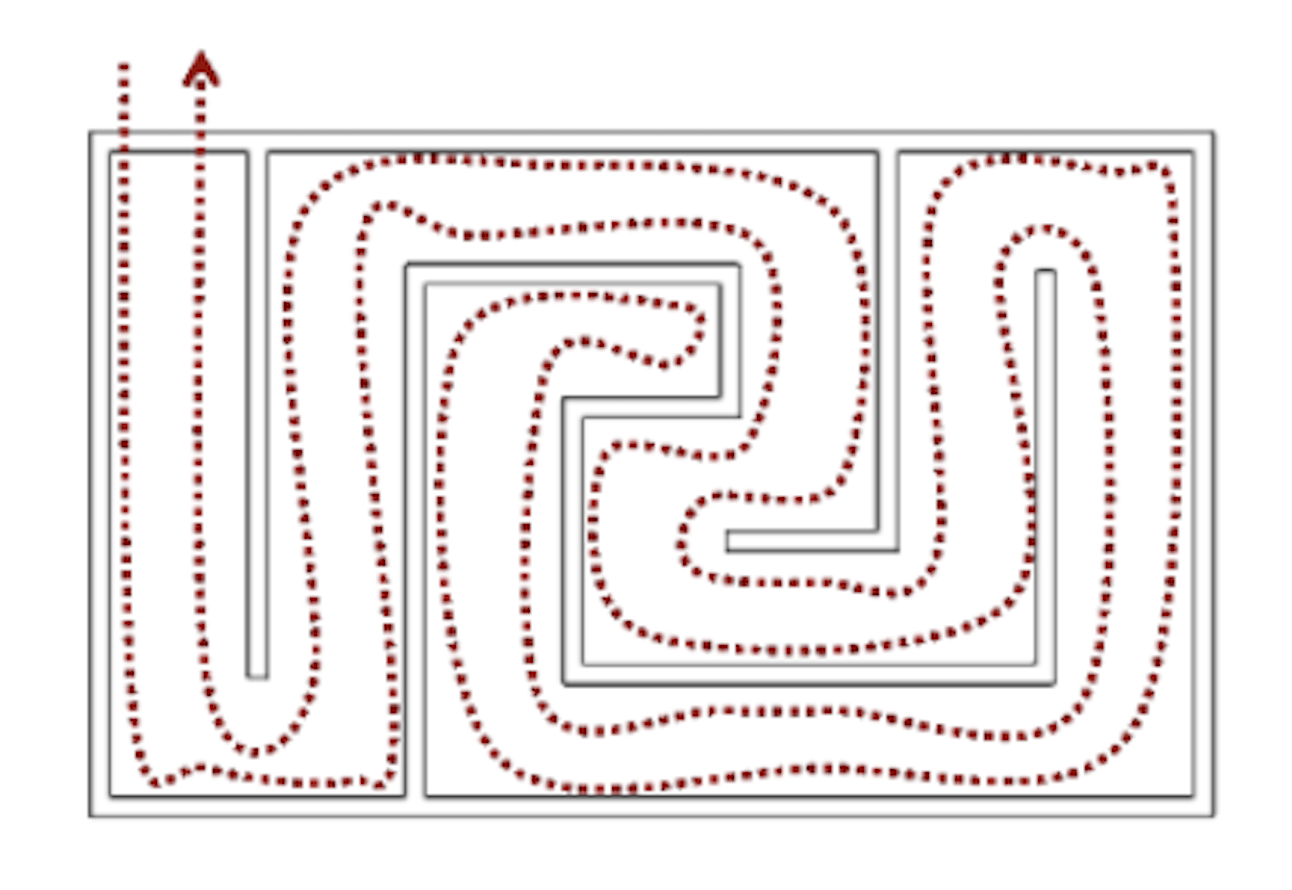
\includegraphics[width=0.5\textwidth]{report/pics/perfect_maze.png}%
        \label{fig:a}%
        }%
    \hfill%
    \subfloat[Labyrinthe imparfait.]{%
        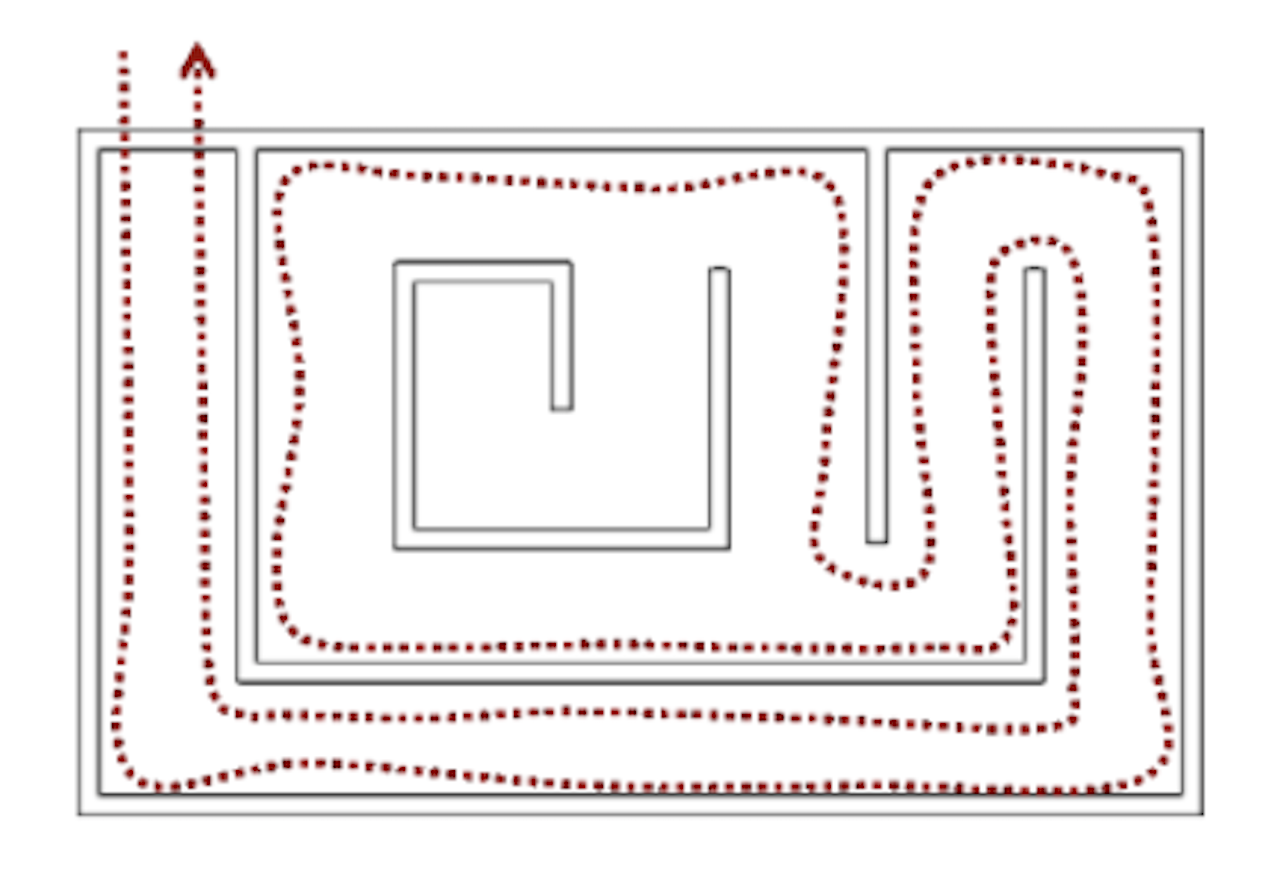
\includegraphics[width=0.5\textwidth]{report/pics/imperfect_maze.png}%
        \label{fig:b}%
        }%
    \caption{Exemple d'un labyrinthe parfait et d'un labyrinthe imparfait.}
\end{figure*}




Dans la suite de ce rapport, nous considérons l'ensemble de nos labyrinthes comme étant de dimension 2 et possédant une tessellation orthogonale. La distinction se feras sur le critère de la topologie, on distinguera alors deux types de labyrinthes : les labyrinthes parfaits et les labyrinthes imparfaits.

\newpage
\section{Introduction à la génération de labyrinthes}
Les algorithmes utilisés pour la génération de labyrinthes suivent un ordre d'étapes prédéfini. Afin de créer des labyrinthes structurés de manière aléatoire, une ou plusieurs étapes de l'algorithme doivent être randomisées (c'est-à-dire que la prise de décision au sein de l'étape doit utiliser une fonction renvoyant un résultat aléatoire). 
Il existe deux approches algorithmiques générales utilisées pour la génération automatisée des labyrinthes. Ces approches sont : l'ajout de murs et la sculpture de passages.
\\
\begin{itemize}
\item\textbf{ Ajout de murs :} Dans cette approche, on se base sur l'ajout de murs pour générer progressivement notre labyrinthe. On démarre d'un labyrinthe vide, puis l'algorithme va placer au fur et à mesure des murs à des positions spécifiques. 
\\
\item\textbf{ Sculpture de passages :} Les algorithmes basés sur cette approche se concentrent sur les chemins et le positionnement des cellules du labyrinthe. On démarre d'une matrice de cellules (une grille complètement remplie de murs), puis l'algorithme de sculpture de passages va alors creuser à travers la grille et détruire certains murs reliant les différentes cellules, ce processus itérative générera au final un labyrinthe.
\end{itemize}



\subsection{Rappels sur la théorie des graphes}
Cette sous-section présente certains principes fondamentaux de la théorie des graphes sur lesquels sont basé les algorithmes de génération de labyrinthes. 
\subsubsection{Graphe}
Un graphe est le concept fondamental dans la théorie des graphes, ce dernier est définie comme étant un triplet  $G = (V, E, \epsilon )$, avec $V$ représentant l'ensemble des sommets, $E$  l'ensemble des arêtes et $\epsilon$ une fonction de mappage appelée relation d'incidence tel que $\epsilon : E	\rightarrow V^2$

\subsubsection{Arbre}
Un arbre est un graphe connexe non orienté ne contenant pas de cycles, c'est-à-dire qu'il existe exactement un seul et unique chemin entre chaque paire de sommets du graphe. Un graphe connexe avec $n$ sommets et $n-1$ arêtes est un arbre.
La suppression de toute les arête entraînerait la perte de connexité du graphe, et l'ajout d'une arête créerait un cycle au sein du graphe.

\subsubsection{Arbre couvrant}
Soit $G$ un graphe. L'arbre couvrant de $G$ est le sous graphe qui est connexe, sans cycle et contient tous les sommets de $G$.


\newpage
\subsection{Théorie des graphes et labyrinthes.}
Sur la figure ci-dessous on peut apercevoir deux labyrinthes. Celui de gauche est un labyrinthe parfait, celui de droite un labyrinthe imparfait (car il contient des boucles). Il existe une autre approche pour visualiser nos labyrinthes. Au lieu de penser aux murs constituants le labyrinthe, nous pouvons penser aux chemins entre les cellules. 
Les chemins à l'intérieur du labyrinthe forment un graphe. Le graphe de chaque labyrinthe est illustré ci-dessous en rouge. \newline
\fig{pics/graphe_theory.png}{12cm}{9cm}
{Géénration d'un labyritnhe 3*3 à l'aide de l'algortihme d'arbre binaire.}{mmcomp}


Dans le cas du labyrinthe imparfait à droite, on va bien qu'il existe une boucle à l'intérieur du graphe.
\fig{pics/graph_theory3.png}{10cm}{7cm}
{Modélisation des labyritnhes sous forme de graphes.}{mmcomp}

De cela, nous arrivons à la conclusion que la génération d'un labyrinthe parfait aléatoire consiste à générer un arbre couvrant aléatoire qui relie toutes les cellules du labyrinthe.
Les différentes procédures et approches utilisées pour la génération d'arbres couvrant forment les bases des différents algorithmes de génération de labyrinthes. 


\section{État de l’art: études des solutions existantes} \label{sec:etatDeLart2}
Dans cette section, nous passons en revue certains des algorithmes les plus populaires utilisés pour la génération de labyrinthes parfaits.
L'ensemble des algorithmes présentés dans cette section suivent l'approche "sculpture de passages" pour générer un labyrinthe. Pour chaque algorithme, on démarre à chaque fois d'une grille remplie de murs, puis l'algorithme se chargera de creuser un chemin parmis ces murs afin de construire son labyrinthe. 
\subsection{Algorithme de Kruskal}
Le générateur de labyrinthe Kruskal est une version aléatoire de l'algorithme de Kruskal. C'est un algorithme qui permet de produire un arbre couvrant pour un graphe (un labyrinthe parfait).
L'algorithme de Kruskal randomnisé pour la génération de labyrinthe fonctionne de la manière suivante :
\newline
\begin{enumerate}
    \item On démarre d'un labyrinthe sous de grille complètement remplie de murs. On regroupe tous les murs séparant les cellules du labyrinthe dans un ensemble.
    \item On choisit un mur à partir de cet ensemble de manière aléatoire et on le supprime du labyrinthe.
    \item On réitère l'opération jusqu'à ce qu'il n'y est plus aucune cellule isolée.
\end{enumerate}
\fig{pics/kruskal.png}{16cm}{12cm}
{Géénration d'un labyritnhe 3*3 à l'aide de l'algortihme de Kruskal.}{mmcomp}


\subsection{Algorithme d'arbre binaire}
L'algorithme de génération de labyrinthes "Arbre Binaire" est l'un des algorithmes les plus simples utilisé pour la génération de labyrinthe parfaits. Une des spécificités de l'algorithme est qu'il n'a pas besoin de sauvegarder en mémoire l'état des cellules du labyrinthe. Il peut construire un labyrinthe entier en regardant une seule cellule à la fois.
Son principe de fonctionnement est très simple :
\newpage
\begin{enumerate}
    \item Pour chaque cellule au sein du labyrinthe, exécuter les étapes deux et trois.
    \item Si ils existent, récupérer les voisins se situant au nord et à l'ouest de la cellule.
    \item On choisit un mur à partir de cet ensemble de manière aléatoire et on le supprime du labyrinthe.
    \item Sélectionner un des voisins de manière aléatoire, et perforer le mur reliant la cellule et le voisin choisit.
\end{enumerate}
\newline
\fig{pics/binary_tree.png}{10cm}{7cm}
{Géénration d'un labyritnhe 3*3 à l'aide de l'algortihme d'arbre binaire.}{mmcomp}



\subsection{Algorithme de Prim}
Dans l'algorithme de Kruskal, on effectuait une sélection aléatoire parmis les murs du labyrinthe qu'on supprimait. L'algorithme de Prim aborde le problème de génération de labyrinthe sous un angle différent, ici, on démarre à partir de n'importe quelle cellule puis à partir de cette cellule l'algorithme va se charger de développer un chemin jusqu'à ce qu'on obtienne un labyrinthe parfait.
L'algorithme de Prim randomnisé pour la génération de labyrinthe suit les étapes suivantes :

\begin{enumerate}
    \item On choisit une cellule de départ de manière aléatoire qu'on ajoute à l'ensemble V.
    \item On choisit une cellule aléatoire C de l'ensemble V dont au moins un des voisins n'appartient pas encore à l'ensemble V. 
    \item On choisit un voisin aléatoir de la cellule C et on perfore le mur reliant ces deux cellules. On ajoute le voisin choisit à l'ensemble V. 
    \item On réitère les étapes deux et trois jusqu'à ce que l'ensemble V contienne toutes les cellules du labyrinthe.
\end{enumerate}
\newpage
Sur la figure ci-dessous on est illustrée la génération d'un labyrinthe à l'aide de l'algorithme de Prim étape par étape. Les cellules appartenant à l'ensemble V (au labyrinthe) sont marquées en blanc, leurs cellules voisines en rose et en jaune on marque à chaque quelle cellule a été chosiit de manière aléatoire.
\fig{pics/prim.png}{16cm}{12cm}
{Géénration d'un labyritnhe 3*3 à l'aide de l'algortihme de Prim.}{mmcomp}

\subsection{Algorithme de Backtracking}
Le Backtracking est une approche et une famille d'algorithmes utilisés pour résoudre des problèmes algorithmiques. Dans cette approche, on construit une solution progressivement et de manière récursive. Dans cette approche, on teste l'ensemble des candidats possibles pour la construction d'une solution, et on revient en arrière (backtracks) dès qu'on détermine qu'un candidat ne peut nous fournir une solution valable. Le Backtracking est un parcours en profondeur sur l'arbre de décision du problème, avec possibilité de revenir en arrière.

\newpage
\section{Comparaison des algorithmes de génération de labyrinthes}

Maintenant qu'on a présenté un ensemble d'algorithmes utilisés pour la génération de labyrinthes parfaits, il faut se décider sur l'algorithme à implémenter afin de générer les labyrinthes dans lequels va évoluer notre Micromouse. Dans cette section, nous présentons les critères et métriques sur lequels on s'est basé afin de comparer les différents algorithmes ainsi que les labyrinthes qu'ils génèrent. Cette section se basent en grande partie sur les recherches et analyses menées par le professeur Jamis Buck dans son livre "Maze pour Programmers"\cite{maze_for_programmers}

\subsubsection{Impasse}
Une impasse est définie comme une cellule qui n'est liée qu'à un seul voisin, c'est à dire une cellule qui ne possède qu'un seul mur perforé, ces autres murs étant fermés.
Un labyrinthe avec peu d'impasses aura tendance à contenir plus de routes secondaires, ce qui aura pour effet de rendre le labyrinthe plus difficile à résoudre. 
D'un point de vu de la Micromouse, et dans le but de tester l'intelligence de cette dernière, on préférera un labyrinthe contenant peu d'impasses afin de pouvoir mettre à épreuve les capacités de décisions de cette dernière. Par exemple, dans un labyrinthe contenant un nombre important d'impasses, on pourrait programmer la Micromouse de sorte qu'elle se contente d'avancer sans réel objectif et qu'elle revienne sur ses pas dans la cas ou elle tombe sur impasse et sauvegarde en mémoire la position de cette dernière. 
Ce n'est clairement pas intéressant comme algorithme de navigation, ce qui nous conforte dans notre choix d'opter pour un algorithme qui génère peu d'impasses.
\newline
La figure suivante montre le nombre moyen d'impasses générées au sein du labyrinthe par différents algorithmes.
\newline
\fig{pics/impasse.png}{16cm}{12cm}
{Moyenne d'impasses engendrées par différents algorithmes de génération de labyrinthes}{mmcomp}
\newline
On constate que l'algorithme de Prim a tendance à produire des labyrinthes où environ 45\% des cellules sont des impasses. En parallèle l'algorithme de Backtracking en génère un nombre beaucoup moins important.


\subsubsection{Variation de directions}
La variation de directions est une mesure de la fréquence à laquelle un passage change de direction. Il est pris comme le pourcentage de cellules avec un passage entrant sur un côté et sortant à gauche ou à droite.
Dans un labyrinthe un faible variation de directions, la majorité des chemins seront des passages droits (horizontaux ou verticaux). Toujours dans l'optique d'utilisation du labyrinthe comme environnement pour la Micromouse, un labyrinthe à faible taux de variation n'est pas intéressant, en effet, l'intelligence de le Micromouse sera mise à l'épreuve lorsque cette dernière devra faire des décisions, l'objectif étant de choisir la direction assurant une solution optimale. Dans le cas de passages en ligne droite, la Micromouse ne fera qu'avancer tout droit en attendant de tomber sur un virage.


\fig{pics/variation_directions}{16cm}{12cm}
{Taux de variation de directions moyens pour différents algorithmes de génération de labyrinthes}{mmcomp}
On s'aperçoit que l'algorithme de Backtracking dispose d'un fréquence de variation de directions de quasiment 50\%, tandis que l'algorithme de Kruskal, de Prim et d'arbre binaire ont des fréquences de variations plus petites.
\subsubsection{Taille du chemin optimal}
Le chemin optimal d'un labyrinthe est définie comme étant le chemin le plus court chemin reliant la cellule de départ et la cellule objectif. Pour calculer la taille du chemin optimal, on commence d'abord par utiliser un algorithme de navigation (résolution du labyrinthe) afin de déterminer quel est le chemin optimal, puis, on calcule le pourcentage de cellules du labyrinthe appartenant à ce chemin.
En général, plus le chemin optimal est long, plus le labyrinthe sera difficile à résoudre.

\fig{pics/plus_long_chemin}{16cm}{12cm}
{Taille moyenne du chemin optimal pour différents algorithmes de génération de labyrinthes}{mmcomp}



\section{Solution proposée et sa mise en œuvre} \label{sec:solution2}
\subsection{Solution implémentée pour la génération de labyrinthes parfaits}
\subsection{Solution implémentée pour la génération de labyrinthes imparfaits}
\paragraph{Chapeau}


\section{Tests et certifications de la solution} \label{sec:test2}

\paragraph{Chapeau}
